\documentclass[12pt]{article}
\author{Mengxiao Zhang-11651502}
    \title{Cpts570-hw2}
    \usepackage{graphicx}
\begin{document}
    \maketitle
    \pagebreak
    \section{Programming and Empirical Analysis Part}
        \subsection{Problem 1}
            \subsubsection{a}
                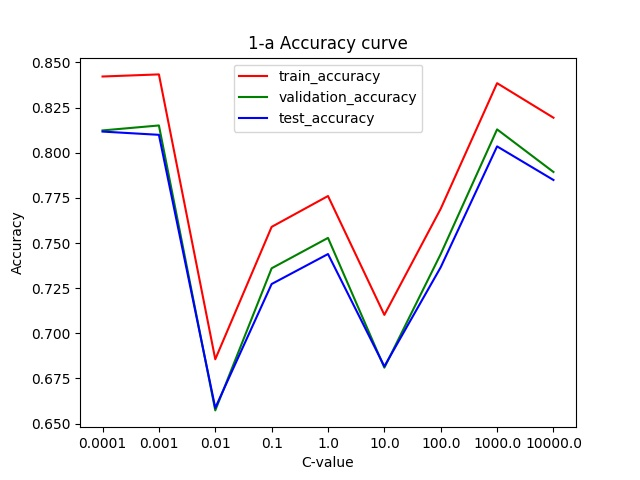
\includegraphics[height=8cm]{part1_a}
                \par Since I use LinearSVC, I cannot plot the
                number of support vectors. And finally I find the best C is 0.001.
            \subsubsection{b}
                \par When C is 0.001, the testing accuracy: 77.69\%.
                \par The corresponding confusion matrix:
                \[
                \left[
                \begin{array}{cccccccccc}
                699 &  9  &  2  & 56 &  16 & 0 & 204 & 1 & 12 & 1  \\
                2   & 943 &  1  & 31 &  6  & 0 & 14  & 1 & 1  & 1  \\
                17  &  6  & 256 & 10 & 258 & 0 & 444 & 0 & 8  & 1  \\
                21  &17   &3    &818 &57   &1  &77   &2  &2   &2\\
                0   & 2   &8    &31  &760  &1  &195  &0  &3   &0\\
                0   &1    &0    &1   &0    &830&2    &98 &12  &56\\
                90  &4    &21   &44  &140  &0  &675  &0  &26  &0\\
                0&0&0&0&0&11&0&970&0&19\\
                4&5&2&8&12&10&34&13&911&1\\
                0&0&0&0&0&7&3&83&0&907
                \end{array}
                \right]
                \]
            \subsubsection{c}
\\ The degree of 2, 3, 4:
\\$'train\ accuracy': array([1., 1., 1.]),$
\\$'validatio\ naccuracy': array ([0.88141667, 0.87016667, 0.8565]),$
\\$'test\ accuracy': array ([0.8755, 0.8671, 0.8477]),$
\\$'Number\ of\ Support\ Vectors': $
\\$array([1841,  216, 2075, 1563, 2119,  959, 2810,  947,  498,  520], dtype=int32),$
\\$array([1539,  169, 1720, 1301, 1815,  941, 2491,  857,  374,  463], dtype=int32),$
\\$array([1362,  149, 1460, 1148, 1556,  993, 2245,  766,  321,  399], dtype=int32)]$
\\ $The\ best\ degree: 2$
\\ According to these data, we can know that with the kernel degree increase, the accuracy of 
validation and test are decrease, and the number of support vectors are also decrease. So that 
the degree 2 is the best one for this poly-kernel SVM
        \subsection{Problem 2}
\\$train\ accuracy: 90.12083333333332 \%$
\\$validation\ accuracy: 89.51666666666667 \%$
\\$test\ accuracy: 90.0 \%$
        \subsection{Problem 3}
            \subsubsection{b}
\\$training\ Accuracy: 100\%$
\\$validation\ Accuracy: 65.00\%$
\\$testing\ Accuracy: 74.28571428571429\%$
            \subsubsection{d}
\\$training\ Accuracy: 86.40167\%$
\\$validation\ Accuracy: 97.014925\%$
\\$test\ Accuracy: 93.9338235\%$
\\ From these data, we can not that with pruning the tree, the training accuracy is decrease 
but validation accuracy and testing accuracy are both increase. I think it is because of the 
overfitting, and when we do the pruning, it become more fittable.
\end{document}
